\section{Tool Implementation}\label{tool-implementation}

Below is the definition of the FoldFeature superclass --- all features
created using Foldlings can override these methods to provide specific
functionality. The , and. It also contains several functions that For
further discussion of the FoldFeature data structure, see
\textbf{\textgreater{}\textgreater{}TODO cite}.

\small
\singlespacing 

\begin{pygmented}{swift}
var horizontalFolds:[Edge] = [] //list of horizontal folds
var featureEdges:[Edge]?        //edges in a feature
var children:[FoldFeature] = [] // children of feature
var drivingFold:Edge? // driving fold of feature
var parent:FoldFeature? // parent of feature
var startPoint:CGPoint?
var endPoint:CGPoint? // start and end touch points

/// splits an edge around the current feature
func splitFoldByOcclusion(edge:Edge) -> [Edge]
{
//by default, return edge whole
return [edge]
}
/// features are leaves if they don't have children
func isLeaf() -> Bool
{
return children.count == 0
}
/// options or modifications that can be made to the current feature
func tapOptions() -> [FeatureOption]?
{
  return [FeatureOption.PrintPlanes, FeatureOption.PrintEdges,
  FeatureOption.ColorPlaneEdges, FeatureOption.PrintSinglePlane]
}
/// whether a feature is drawn over a fold, determines whether 
/// a fold can be the driving fold for a feature
  func featureSpansFold(fold:Edge)->Bool
{
  return false
}
/// returns and calculates planes in a feature
func getFeaturePlanes()-> [Plane]{
  return featurePlanes
}
/// whether a feature contains a point
/// needs to be overridden by subclasses
func containsPoint(point:CGPoint) -> Bool{
  return self.boundingBox()?.contains(point) ?? false
}
\end{pygmented}

\doublespacing
\normalsize

Of these functions, the most complex are \emph{featureSpansFold} and
\emph{splitFoldByOcclusion}. \emph{FeatureSpansFold} is implemented
depending on

\subsection{Box Fold}\label{box-fold}

talk about occlusion

talk about feature spans fold

\subsubsection{FreeForm}\label{freeform}

A freeform shape consists of a series of interpolation points through
which a we construct a bezier curve using the Catmull-Rom algorithm.
\textbf{\textgreater{}\textgreater{}TODO:CITE} We capture interpolation
points as a function of touch velocity. That is, when the user draws
more quickly, we capture more interpolation points closer together. This
allows us to capture the entire drawing with a similar level of detail
throughout, and correct for the gesture recognizer sending relatively
more frequent updates when the touch is moving more slowly.

However, the catmull-Rom algorithm only draws a full path when the start
and end points of the curve are coincident. We use an alpha value of
1.0, which we found to be the closest to the intended touch shape
through informal user studies.

When a freeform shape has a driving fold, we must add

\begin{figure}[htbp]
\centering
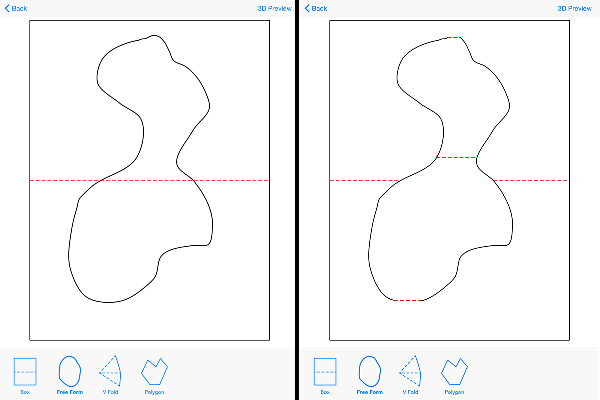
\includegraphics{figures/41_Tech_Tool_Implementation/truncationBeforeAfter.pdf}
\caption{}
\end{figure}

\small
\singlespacing 

\begin{pygmented}{swift}
func truncateWithFolds()
\end{pygmented}

\doublespacing
\normalsize

\begin{algorithm}[H]

\KwData{\textit{path}, the bezier path for the freeform shape}

\KwResult{edges for truncated shape}

create \textit{scanline} at top of bounding box for \textit{feature}

\While{\textit{scanline} above bottom of \textit{feature}}{

\textit{intercepts} $\leftarrow$ intersection points between \textit{scanline} and \textit{path}

\If{\textit{intercepts} not nil}{

    \textit{fragments} $\leftarrow$ \textit{path} split by \textit{intercepts}
    
    \ForEach{\textit{fragment} in \textit{fragments}}{
    
    \If{\textit{fragment} center is above top fold or below bottom fold}{
    
    remove \textit{fragment} from \textit{fragments}
    
    }
    
    }
    
\bf{break}

}

translate \textit{scanline} down

}
 
repeat \textit{scanline} operation from bottom to find bottom fold
    
calculate middle fold position
    
\textit{folds} $\leftarrow$ top, middle, and bottom folds
    
\Return{\textit{folds} + \textit{fragments}}  

\caption{Truncation}
\end{algorithm}

talk about bitmap intersection for scanline

Essentially, we use a bitmap approximation of the intersection point
between bezier paths, because calculating intersections between
arbitrary curves is computationally more expensive. We use this fast
approximation to .

\textbf{\textgreater{}\textgreater{}TODO DISCUSSION OF SPLITTING} talk
about splitting algorithm. Recursively subdivide

\subsubsection{Polygon}\label{polygon}

Polygons are very similar to freeform shapes. The main difference
between polygon and freeform shapes is that the intersection tests for
polygons are much cheaper. For intersections between polygons, we can
use a simple system of equations, rather than the bitmap intersection
technique described above.

The interpolation points are vertices of the polygon

\subsubsection{V-Fold}\label{v-fold}

Geometric constraints as described in angle calculation, path splitting

\subsection{Self-intersecting Paths}\label{self-intersecting-paths}

In order to be rendered by SceneKit in 3D, paths cannot have self
intersections. Thus, we attempt to repair self-intersecting paths when
adding features to the sketch. Self intersections occur in two ways: the
user creates a self-intersecting path, or paths self-intersect as a
result of imprecision in performing intersections or capturing touch
interpolation points. ~ ~

\begin{figure}[htbp]
\centering
\includegraphics{figures/41_Tech_Tool_Implementation/loopBeforeAfter.pdf}
\caption{}
\end{figure}

\begin{algorithm}[H]

 \textit{segments} $\leftarrow$ bezier path discretized into straight line segments using adaptive subdivision 
 
 \textit{sanitizedSegments} $\leftarrow$ empty array
  
 \For{\textit{i} $\leftarrow$ 0; \textit{i} < \textit{segments}.length; \textit{i}++}{

//compare with all segments after current segment

\For{\textit{j}  $\leftarrow$ \textit{i}; \textit{j} < \textit{segments}.length; \textit{j}++}{

\If{\textit{segments}[\textit{i}] intersects \textit{segments}[\textit{j}]}{

    remove \textit{segments}[\textit{i}..\textit{j}] from path

    \textit{i} $\leftarrow$ \textit{j}  //skip segments inbetween intersecting segments, thereby repairing the "loop"

}

\textit{sanitizedSegments}.append(\textit{segments}[\textit{i}])

}

}
 
 \Return{sanitizedSegments} \
 
\caption{Self-intersecting path repair}
\end{algorithm}

A convoluted design with many overlapping self intersections can fail to
resolve to a valid shape. In cases where our algorithm fails, we display
an error and do not add the feature to the sketch.

\begin{figure}[htbp]
\centering
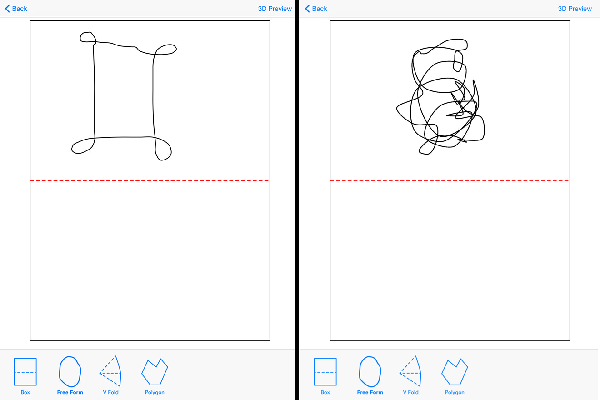
\includegraphics{figures/41_Tech_Tool_Implementation/succeedFailSelfIntersections.pdf}
\caption{}
\end{figure}
